%%%%%%%%%%%%%%%%%%%%%%%%%%%%%%%%%%%%%%%%%%%%%%%%%%%%%%%%%%%%%%%%%%%%%%%%%%%%%%%%
%%%%%%%%%%%%%%%%%%%%%%%%%%%%%%%%%%%%%%%%%%%%%%%%%%%%%%%%%%%%%%%%%%%%%%%%%%%%%%%%
%
% A general frame for lecture slides and lecture notes in one file
% using LaTeX beamer
%
%%%%%%%%%%%%%%%%%%%%%%%%%%%%%%%%%%%%%%%%%%%%%%%%%%%%%%%%%%%%%%%%%%%%%%%%%%%%%%%%
%%%%%%%%%%%%%%%%%%%%%%%%%%%%%%%%%%%%%%%%%%%%%%%%%%%%%%%%%%%%%%%%%%%%%%%%%%%%%%%%
\documentclass[ignorenonframetext,11pt]{beamer}
%\usepackage[ngerman]{babel}
%\usepackage[T1]{fontenc}
\usepackage[utf8]{inputenc}
\usepackage{lmodern}
\usepackage{amsmath,amssymb,amsfonts}


% only presentation
\mode<presentation>
{
  \usetheme{default}
%  \usecolortheme{crane}
  \setbeamercovered{transparent}
%  \setlength{\parindent}{0pt}
%  \setlength{\parskip}{1.35ex plus 0.5ex minus 0.3ex}
%  \usefonttheme{structuresmallcapsserif}
  \usefonttheme{structurebold}
  \setbeamertemplate{theorems}[numbered]
  \usepackage{amscd}
}

% all after
\usepackage{tikz}
\usetikzlibrary{patterns}
\usepackage{pgfplots,adjustbox}
\usepackage{eurosym}
\usepackage{graphicx}
\usepackage{multimedia}
\usepackage{psfrag}
\usepackage{listings}
\lstset{language=C++, basicstyle=\ttfamily,
  keywordstyle=\color{black}\bfseries, tabsize=4, stringstyle=\ttfamily,
  commentstyle=\it, extendedchars=true, escapeinside={/*@}{@*/}}
\usepackage{curves}
%\usepackage{epic}
\usepackage{calc}
%\usepackage{picinpar}
%\usepackage{fancybox}
%\usepackage{xspace}
\usepackage{enumerate}
\usepackage{algpseudocode}
\usepackage{color}
\usepackage{bold-extra}
\usepackage{bm}
\usepackage{stmaryrd}
%\usepackage[squaren]{SIunits}
\usepackage{nicefrac}

\usepackage{fancyvrb,bbm,xspace}
\usepackage{lmodern}
\usepackage{fancyvrb,bbm,xspace}
\usepackage[binary-units]{siunitx}
\usepackage{xcolor,tabu}

\definecolor{niceblue}{rgb}{0.122,0.396,0.651}   %% 31, 101, 166 or #1F65A6
\definecolor{niceorange}{RGB}{255,205,86}        %% #FFCD56
\definecolor{nicered}{RGB}{220,20,60}                      %% rgb(220, 20, 60)
\definecolor{niceteal}{HTML}{00A9AB}
\definecolor{niceviolet}{HTML}{820080}

\definecolor{niceblueLight}{HTML}{91CAFB}
\definecolor{niceblueVeryLight}{HTML}{DDEFFF}

\usepackage{dsfont}

%\newcommand{\hlineabove}{\rule{0pt}{2.6ex}}
%\newcommand{\hlinebelow}{\rule[-1.2ex]{0pt}{0pt}}

%\usecolortheme[RGB={37,75,123}]{structure}
% \definecolor{structurecolor}{rgb}{0.905,0.318,0.071}

% \setbeamercolor{frametitle}{fg=black,bg=}
% \setbeamercolor{sidebar left}{fg=,bg=}

% \setbeamertemplate{headline}{\vskip4em}
% \setbeamersize{sidebar width left=.9cm}

% \setbeamertemplate{navigation symbols}{}
%\setbeamertemplate{blocks}[rounded][shadow=true]
%\setbeamertemplate{itemize items}[square]

\mode<presentation>
{
\theoremstyle{definition}
}
\newtheorem{Def}{Definition}%[section]
\newtheorem{Exm}[Def]{Example}
\newtheorem{Lem}[Def]{Lemma}
\newtheorem{Rem}[Def]{Remark}
\newtheorem{Rul}[Def]{Rule}
\newtheorem{Thm}[Def]{Theorem}
\newtheorem{Cor}[Def]{Corollary}
\newtheorem{Obs}[Def]{Observation}
\newtheorem{Ass}[Def]{Assumption}
\newtheorem{Pro}[Def]{Property}
\newtheorem{Alg}[Def]{Algorithm}
\newtheorem{Prp}[Def]{Proposition}
\newtheorem{Lst}[Def]{Listing}

% Delete this, if you do not want the table of contents to pop up at
% the beginning of each subsection:
\AtBeginSection[]
{
  \begin{frame}<beamer>
    \frametitle{Contents}
    \tableofcontents[sectionstyle=show/shaded,subsectionstyle=hide/hide/hide]
%\tableofcontents[currentsection]
  \end{frame}
}

% Title definition
\mode<presentation>
{
  \title{DUNE PDELab Tutorial 04\\
  {\small Finite Elements for the Wave Equation}}
  \author{Peter Bastian \and Steffen Müthing}
  \institute[]
  {
   Interdisziplinäres Zentrum für Wissenschaftliches Rechnen\\
   Im Neuenheimer Feld 205, D-69120 Heidelberg \\[6pt]
  }
  \date[\today]{\today}
}


% logo nach oben
\mode<presentation>
{
% No navigation symbols and no lower logo
\setbeamertemplate{sidebar right}{}

% logo
\newsavebox{\logobox}
\sbox{\logobox}{%
    \hskip\paperwidth%
    \rlap{%
      % putting the logo should not change the vertical possition
      \vbox to 0pt{%
        \vskip-\paperheight%
        \vskip0.35cm%
        \llap{\insertlogo\hskip0.1cm}%
        % avoid overfull \vbox messages
        \vss%
      }%
    }%
}

\addtobeamertemplate{footline}{}{%
    \usebox{\logobox}%
}
}

%%%%%%%%%%%%%%%%%%%%%%%%%%%%%%%%%%%%%%%%%%%%%%%%%%%%%%%%%%%%%%%%%%%%%%%%%%%%%%%%
%%%%%%%%%%%%%%%%%%%%%%%%%%%%%%%%%%%%%%%%%%%%%%%%%%%%%%%%%%%%%%%%%%%%%%%%%%%%%%%%
%
% now comes the individual stuff lecture by lecture
%
%%%%%%%%%%%%%%%%%%%%%%%%%%%%%%%%%%%%%%%%%%%%%%%%%%%%%%%%%%%%%%%%%%%%%%%%%%%%%%%%
%%%%%%%%%%%%%%%%%%%%%%%%%%%%%%%%%%%%%%%%%%%%%%%%%%%%%%%%%%%%%%%%%%%%%%%%%%%%%%%%

\begin{document}

\frame{\titlepage}

%%%%%%%%%%%%%%%%%%%%%%%%%%%%%%%%%%%%%%%%%%%%%%%%%%%%%%%%%%%%%%%%%%%%%%%%%%%%%%%%
%%%%%%%%%%%%%%%%%%%%%%%%%%%%%%%%%%%%%%%%%%%%%%%%%%%%%%%%%%%%%%%%%%%%%%%%%%%%%%%%


\begin{frame}
\frametitle{Example Problem}
 In this tutorial we solve the wave equation formulated as a first order
in time system. This way the example serves as a model for the
treatment of systems of partial differential equations in PDELab.

\begin{subequations}
\label{eq:WaveEquation}
\begin{align}
\partial_{tt} u-c^2\Delta u  &= 0 &&\text{in $\Omega\times\Sigma$},\\
u &= 0 &&\text{on $\partial\Omega$},\\
u &= q &&\text{at $t=0$},\\
\partial_t u &= w &&\text{at $t=0$},
\end{align}
\end{subequations}
where $c$ is the speed of sound.
\end{frame}
\begin{frame}
Renaming $u_0=u$ and introducing $u_1=\partial_t u_0 =\partial_t u$ we can write the wave equation as a system of two equations:
\begin{subequations}
\label{eq:SystemForm1}
\begin{align}
\partial_t u_1 - c^2\Delta u_0 &=0 &&\text{in $\Omega\times\Sigma$}, \label{eq:2a}\\
\partial_t u_0 - u_1 &=0 &&\text{in $\Omega\times\Sigma$}, \label{eq:2b}\\
u_0 &= 0 &&\text{on $\partial\Omega$},\\
u_1 &= 0 &&\text{on $\partial\Omega$},\\
u_0 &= q &&\text{at $t=0$},\\
u_1 &= w &&\text{at $t=0$}.
\end{align}
\end{subequations}
Since $u_0=u=0$ on the boundary we also have $\partial_t u = u_1 = 0$ on the boundary.
Alternatively, omit the boundary condition on $u_1$.
\end{frame}


\begin{frame}
\frametitle{Alternative Formulations (I)}
Eriksson et al. in \cite{Eriksson} apply the Laplacian to
equation \eqref{eq:2b}
\begin{equation}
\Delta \partial_t u_0 - \Delta u_1 = 0
\end{equation} \label{eq:Eriksson}
which has advantages for energy conservation but requires additional smoothness
properties.
\end{frame}

\begin{frame}
\frametitle{Alternative Formulations (II)}
Introduce the abbreviations
$q=\partial_t u$ and $w=-\nabla u$, so $\partial_{tt} u - c^2 \Delta u =
\partial_{tt} u - c^2 \nabla\cdot\nabla u = \partial_{t} q + c^2 \nabla\cdot w = 0$.
Taking partial derivatives of the introduced variables we obtain $\partial_{x_i} q=
\partial_{x_i} \partial_t u = \partial_t \partial_{x_i}  u = - \partial_t w_i$. This results
in a first-order hyperbolic system of PDEs for $q$ and $w$
\begin{align*}
\partial_t q + c^2 \nabla\cdot w &= 0\\
\partial_t w + \nabla q &= 0
\end{align*}
which are called equations of linear acoustics \cite{LeVeque}. This formulation
is physically more relevant. It can be modified to handle discontinuous material
properties and supports upwind finite volume methods.
\end{frame}


\begin{frame}
\frametitle{Weak Formulation}

Multiplying \eqref{eq:2a}
with the test function $v_0$ and \eqref{eq:2b} with the test function $v_1$
and using integration by parts we arrive at the weak formulation: Find $(u_0(t),u_1(t))\in
U_0\times U_1$ s.t.
\begin{align}
  d_t (u_1,v_0)_{0,\Omega} + c^2 (\nabla u_0, \nabla v_0)_{0,\Omega} &=
  0 \quad \forall v_0 \in U_0 \notag \\
  d_t (u_0,v_1)_{0,\Omega} - (u_1,v_1)_{0,\Omega} &= 0 \quad \forall
  v_1 \in U_1 \label{eq:WeakFormSystem}
\end{align}
where we used the notation of the $L^2$ inner product $(u,v)_{0,\Omega} = \int_\Omega
u v \, dx$.
\end{frame}

\begin{frame}
An equivalent formulation to (\ref{eq:WeakFormSystem}) that
hides the system structure reads as follows:
\begin{equation}
\label{eq:WeakForm}
\begin{split}
d_t &\left[ (u_0,v_1)_{0,\Omega} + (u_1,v_0)_{0,\Omega}\right] \\
&\hspace{6mm}+ \left[ c^2 (\nabla u_0,\nabla v_0)_{0,\Omega} -(u_1,v_1)_{0,\Omega} \right] = 0
\quad \forall (v_0,v_1)\in U_0\times U_1
\end{split}
\end{equation}
With the latter we readily identify the temporal and spatial residual
forms:
\begin{align}
m^{\text{WAVE}}((u_0,u_1),(v_0,v_1)) &= (u_0,v_1)_{0,\Omega} + (u_1,v_0)_{0,\Omega},
\label{eq:TemporalResForm}\\
r^{\text{WAVE}}((u_0,u_1),(v_0,v_1)) &= c^2 (\nabla u_0,\nabla
v_0)_{0,\Omega} - (u_1,v_1)_{0,\Omega} \; . \label{eq:SpatialResForm}
\end{align}
\end{frame}


\begin{frame}{Trees of Function spaces}
  \begin{columns}
    \begin{column}{0.6\textwidth}
$U = \bigl(V(\Omega_S)\bigr)^d \times P(\Omega_S) \times \Phi(\Omega_D)$

\begin{itemize}
\item Computer science way of representing mathematical  expressions: \structure{Trees}
\item Expose internal nodes to users
  \begin{itemize}
  \item {\small Enable recursive bottom-up construction}
  \item {\small Extract subtrees to pass to legacy subproblem code}
  \end{itemize}
\item Tree structure mostly static after construction
  \begin{itemize}
  \item {\small Nodes are C++ templates with children as template arguments}
  \item {\small Allows extensive compiler optimizations, including inlining of tree traversals}
  \end{itemize}
\end{itemize}

    \end{column}
    \begin{column}{0.4\textwidth}
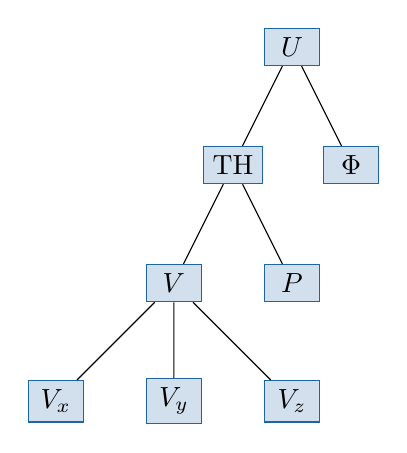
\begin{tikzpicture}
    [every node/.style={draw=niceblue,fill=niceblue!20, minimum width=.7cm}]
  \node {$U$}
  child {
    node {TH}
      child {
        node  {$V$}
        child {
          node  {$V_x$}
        }
        child {
          node  {$V_y$}
        }
        child {
          node  {$V_z$}
        }
      }
      child {
        node  {$P$}
      }
    }
  child {
    node {$\Phi$}
  };
\end{tikzpicture}

    \end{column}
  \end{columns}


\end{frame}

\begin{frame}{Linear Algebra}

    Given an assembled residual $r = \mathcal{R}(\vec{u_0})$ and its Jacobian $A = \nabla\mathcal{R}_h$, we have to solve the linear problem
    \begin{equation*}
      A z = r
    \end{equation*}
    to obtain a correction and calculate $u = u_0 - z$.\\
  \emph{Several options}
  \begin{description}
  \item[Monolithic solve] of $A z = r$
  \end{description}
  \begin{itemize}
  \item No stability problems
  \item Often very difficult with standard iterative solvers
  \end{itemize}
  \begin{description}
  \item[Subdomain Iteration] Exploit problem structure
  \end{description}
\begin{equation*}
  \begin{pmatrix}
    A_L & 0 \\
    0  & A_R \\
  \end{pmatrix}
  \begin{pmatrix}
    z_L \\ z_R \\
  \end{pmatrix}
  =
  \begin{pmatrix}
    r_L \\ r_R \\
  \end{pmatrix}
\end{equation*}
\begin{itemize}
\item Stability can be problematic
\item Does not require monolithic code base
\item Matrix / vector data structures must contain structure for good performance
\end{itemize}
\end{frame}



\begin{frame}{Index Merging -- Example}
  \begin{columns}
    \begin{column}{0.5\textwidth}
      \begin{itemize}
      \item Two $Q_1$ spaces on common mesh
      \item Each space has canonical order defined by vertex iteration
      \item Two merging strategies
        \structure{Lexicographic:} Preserve structure of individual problems, separate matrix blocks for coupling\\
        \structure{Interleaved:} Regard problem as vector-valued version of scalar problem
      \end{itemize}
% \tikzexternalenable
% \resizebox{\textwidth}{!}{
% \input{tikz/dofs/lexicographicmatrix.tex}
% 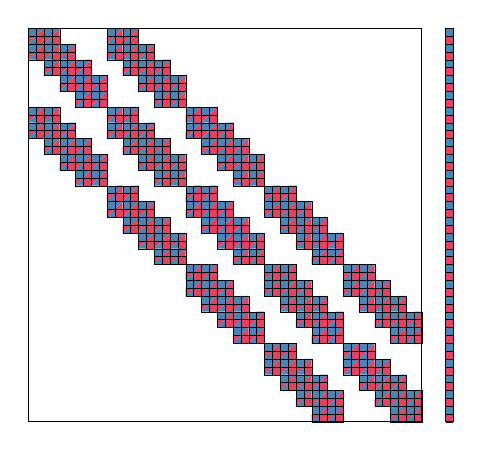
\begin{tikzpicture}

\colorlet{ca}{niceblue!80}
\colorlet{cb}{nicered!80}
\colorlet{cc}{niceorange!90}
\colorlet{cd}{niceviolet!60}

%%% Local Variables:
%%% mode: latex
%%% TeX-master: "../../diss-main"
%%% End:


\foreach \x / \y in {0/0, 0/2, 0/10, 0/12, 2/0, 2/2, 2/4, 2/10,
  2/12, 2/14, 4/2, 4/4, 4/6, 4/12, 4/14, 4/16, 6/4, 6/6, 6/8,
  6/14, 6/16, 6/18, 8/6, 8/8, 8/16, 8/18, 10/0, 10/2, 10/10,
  10/12, 10/20, 10/22, 12/0, 12/2, 12/4, 12/10, 12/12, 12/14,
  12/20, 12/22, 12/24, 14/2, 14/4, 14/6, 14/12, 14/14, 14/16,
  14/22, 14/24, 14/26, 16/4, 16/6, 16/8, 16/14, 16/16, 16/18,
  16/24, 16/26, 16/28, 18/6, 18/8, 18/16, 18/18, 18/26, 18/28,
  20/10, 20/12, 20/20, 20/22, 20/30, 20/32, 22/10, 22/12, 22/14,
  22/20, 22/22, 22/24, 22/30, 22/32, 22/34, 24/12, 24/14, 24/16,
  24/22, 24/24, 24/26, 24/32, 24/34, 24/36, 26/14, 26/16, 26/18,
  26/24, 26/26, 26/28, 26/34, 26/36, 26/38, 28/16, 28/18, 28/26,
  28/28, 28/36, 28/38, 30/20, 30/22, 30/30, 30/32, 30/40, 30/42,
  32/20, 32/22, 32/24, 32/30, 32/32, 32/34, 32/40, 32/42, 32/44,
  34/22, 34/24, 34/26, 34/32, 34/34, 34/36, 34/42, 34/44, 34/46,
  36/24, 36/26, 36/28, 36/34, 36/36, 36/38, 36/44, 36/46, 36/48,
  38/26, 38/28, 38/36, 38/38, 38/46, 38/48, 40/30, 40/32, 40/40,
  40/42, 42/30, 42/32, 42/34, 42/40, 42/42, 42/44, 44/32, 44/34,
  44/36, 44/42, 44/44, 44/46, 46/34, 46/36, 46/38, 46/44, 46/46,
  46/48, 48/36, 48/38, 48/46, 48/48}
{
  \filldraw[fill=ca,ultra thin] (0.1*\x,-0.1*\y) rectangle ++(0.1,-0.1);
}

\foreach \x / \y in {1/1, 1/3, 1/11, 1/13, 3/1, 3/3, 3/5, 3/11,
  3/13, 3/15, 5/3, 5/5, 5/7, 5/13, 5/15, 5/17, 7/5, 7/7, 7/9,
  7/15, 7/17, 7/19, 9/7, 9/9, 9/17, 9/19, 11/1, 11/3, 11/11,
  11/13, 11/21, 11/23, 13/1, 13/3, 13/5, 13/11, 13/13, 13/15,
  13/21, 13/23, 13/25, 15/3, 15/5, 15/7, 15/13, 15/15, 15/17,
  15/23, 15/25, 15/27, 17/5, 17/7, 17/9, 17/15, 17/17, 17/19,
  17/25, 17/27, 17/29, 19/7, 19/9, 19/17, 19/19, 19/27, 19/29,
  21/11, 21/13, 21/21, 21/23, 21/31, 21/33, 23/11, 23/13, 23/15,
  23/21, 23/23, 23/25, 23/31, 23/33, 23/35, 25/13, 25/15, 25/17,
  25/23, 25/25, 25/27, 25/33, 25/35, 25/37, 27/15, 27/17, 27/19,
  27/25, 27/27, 27/29, 27/35, 27/37, 27/39, 29/17, 29/19, 29/27,
  29/29, 29/37, 29/39, 31/21, 31/23, 31/31, 31/33, 31/41, 31/43,
  33/21, 33/23, 33/25, 33/31, 33/33, 33/35, 33/41, 33/43, 33/45,
  35/23, 35/25, 35/27, 35/33, 35/35, 35/37, 35/43, 35/45, 35/47,
  37/25, 37/27, 37/29, 37/35, 37/37, 37/39, 37/45, 37/47, 37/49,
  39/27, 39/29, 39/37, 39/39, 39/47, 39/49, 41/31, 41/33, 41/41,
  41/43, 43/31, 43/33, 43/35, 43/41, 43/43, 43/45, 45/33, 45/35,
  45/37, 45/43, 45/45, 45/47, 47/35, 47/37, 47/39, 47/45, 47/47,
  47/49, 49/37, 49/39, 49/47, 49/49}
{
  \filldraw[fill=cb,ultra thin] (0.1*\x,-0.1*\y) rectangle ++(0.1,-0.1);
}

\foreach \x / \y in {0/1, 0/3, 0/11, 0/13, 2/1, 2/3, 2/5, 2/11,
  2/13, 2/15, 4/3, 4/5, 4/7, 4/13, 4/15, 4/17, 6/5, 6/7, 6/9,
  6/15, 6/17, 6/19, 8/7, 8/9, 8/17, 8/19, 10/1, 10/3, 10/11,
  10/13, 10/21, 10/23, 12/1, 12/3, 12/5, 12/11, 12/13, 12/15,
  12/21, 12/23, 12/25, 14/3, 14/5, 14/7, 14/13, 14/15, 14/17,
  14/23, 14/25, 14/27, 16/5, 16/7, 16/9, 16/15, 16/17, 16/19,
  16/25, 16/27, 16/29, 18/7, 18/9, 18/17, 18/19, 18/27, 18/29,
  20/11, 20/13, 20/21, 20/23, 20/31, 20/33, 22/11, 22/13, 22/15,
  22/21, 22/23, 22/25, 22/31, 22/33, 22/35, 24/13, 24/15, 24/17,
  24/23, 24/25, 24/27, 24/33, 24/35, 24/37, 26/15, 26/17, 26/19,
  26/25, 26/27, 26/29, 26/35, 26/37, 26/39, 28/17, 28/19, 28/27,
  28/29, 28/37, 28/39, 30/21, 30/23, 30/31, 30/33, 30/41, 30/43,
  32/21, 32/23, 32/25, 32/31, 32/33, 32/35, 32/41, 32/43, 32/45,
  34/23, 34/25, 34/27, 34/33, 34/35, 34/37, 34/43, 34/45, 34/47,
  36/25, 36/27, 36/29, 36/35, 36/37, 36/39, 36/45, 36/47, 36/49,
  38/27, 38/29, 38/37, 38/39, 38/47, 38/49, 40/31, 40/33, 40/41,
  40/43, 42/31, 42/33, 42/35, 42/41, 42/43, 42/45, 44/33, 44/35,
  44/37, 44/43, 44/45, 44/47, 46/35, 46/37, 46/39, 46/45, 46/47,
  46/49, 48/37, 48/39, 48/47, 48/49}
{
  \fill[cb] (0.1*\x,-0.1*\y) -- ++(0.1,0) -- ++(-0.1,-0.1) --cycle;
  \fill[ca] (0.1*\x+0.1,-0.1*\y) -- ++(0,-0.1) -- ++(-0.1,0) --cycle;
  \draw[ultra thin] (0.1*\x,-0.1*\y) rectangle ++(0.1,-0.1);
}

\foreach \x / \y in {1/0, 1/2, 1/10, 1/12, 3/0, 3/2, 3/4, 3/10,
  3/12, 3/14, 5/2, 5/4, 5/6, 5/12, 5/14, 5/16, 7/4, 7/6, 7/8,
  7/14, 7/16, 7/18, 9/6, 9/8, 9/16, 9/18, 11/0, 11/2, 11/10,
  11/12, 11/20, 11/22, 13/0, 13/2, 13/4, 13/10, 13/12, 13/14,
  13/20, 13/22, 13/24, 15/2, 15/4, 15/6, 15/12, 15/14, 15/16,
  15/22, 15/24, 15/26, 17/4, 17/6, 17/8, 17/14, 17/16, 17/18,
  17/24, 17/26, 17/28, 19/6, 19/8, 19/16, 19/18, 19/26, 19/28,
  21/10, 21/12, 21/20, 21/22, 21/30, 21/32, 23/10, 23/12, 23/14,
  23/20, 23/22, 23/24, 23/30, 23/32, 23/34, 25/12, 25/14, 25/16,
  25/22, 25/24, 25/26, 25/32, 25/34, 25/36, 27/14, 27/16, 27/18,
  27/24, 27/26, 27/28, 27/34, 27/36, 27/38, 29/16, 29/18, 29/26,
  29/28, 29/36, 29/38, 31/20, 31/22, 31/30, 31/32, 31/40, 31/42,
  33/20, 33/22, 33/24, 33/30, 33/32, 33/34, 33/40, 33/42, 33/44,
  35/22, 35/24, 35/26, 35/32, 35/34, 35/36, 35/42, 35/44, 35/46,
  37/24, 37/26, 37/28, 37/34, 37/36, 37/38, 37/44, 37/46, 37/48,
  39/26, 39/28, 39/36, 39/38, 39/46, 39/48, 41/30, 41/32, 41/40,
  41/42, 43/30, 43/32, 43/34, 43/40, 43/42, 43/44, 45/32, 45/34,
  45/36, 45/42, 45/44, 45/46, 47/34, 47/36, 47/38, 47/44, 47/46,
  47/48, 49/36, 49/38, 49/46, 49/48}
{
  \fill[ca] (0.1*\x,-0.1*\y) -- ++(0.1,0) -- ++(-0.1,-0.1) --cycle;
  \fill[cb] (0.1*\x+0.1,-0.1*\y) -- ++(0,-0.1) -- ++(-0.1,0) --cycle;
  \draw[ultra thin] (0.1*\x,-0.1*\y) rectangle ++(0.1,-0.1);
}

\foreach \x in {0,1,...,24}
{
  \fill[ca] (5.3,-0.2*\x) rectangle ++(0.1,-0.1);
  \fill[cb] (5.3,-0.2*\x-0.1) rectangle ++(0.1,-0.1);
}

\draw (5.3,0) rectangle ++(0.1,-5);

\foreach \x in {0,1,...,50}
{
  %\draw (0.1*\x,0) -- ++(0,-5);
  %\draw (0,-0.1*\x) -- ++(5,0);
  \draw[ultra thin] (5.3,-0.1*\x) -- ++(0.1,0);
}

\draw (0,0) rectangle (5,-5);

\end{tikzpicture}


%%% Local Variables:
%%% mode: latex
%%% TeX-master: "../../diss-main"
%%% End:

% }
% \tikzexternaldisable

    \end{column}
    \begin{column}{0.5\textwidth}
{\Large
\begin{equation*}
U = U_1 \times U_2
\end{equation*}}\vspace*{.5em}
\resizebox{\textwidth}{!}{
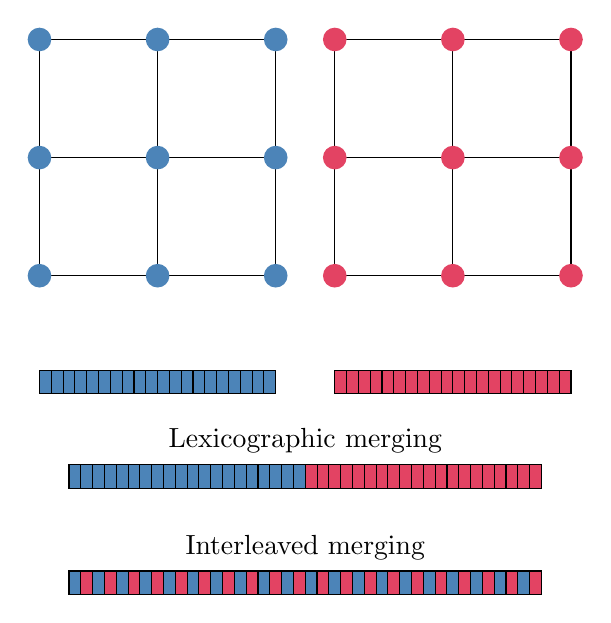
\begin{tikzpicture}[scale=1.5]

\colorlet{ca}{niceblue!80}
\colorlet{cb}{nicered!80}
\colorlet{cc}{niceorange!90}
\colorlet{cd}{niceviolet!60}

%%% Local Variables:
%%% mode: latex
%%% TeX-master: "../../diss-main"
%%% End:


\foreach \c / \i in {ca/0,cb/2.5}
{

\foreach \x in {0,1}
  \foreach \y in {0,1}
  {
    \draw (\x+4 + \i,\y) rectangle ++(1,1);
  }

\foreach \x in {0,1,2}
  \foreach \y in {0,1,2}
  {
    \fill[\c] (\x+4 + \i,\y) circle (0.1);
  }

\filldraw[fill=\c] (4 + \i,-1) rectangle ++(2,0.2);
\foreach \x in {0.1,0.2,...,1.9}
  \draw (4 + \i+\x,-1) -- ++(0,0.2);

\filldraw[fill=\c] ((4.25 + 0.8*\i,-1.8) rectangle ++(2,0.2);
 \foreach \x in {0.1,0.2,...,1.9}
   \draw (4.25 + 0.8*\i +\x,-1.8) -- ++(0,0.2);
}

\draw (6.25,-1.4) node {Lexicographic merging};

\draw (6.25,-2.3) node {Interleaved merging};

\foreach \x in {0,0.1,...,1.91}
{
  \fill[color=ca] (4.25+2*\x,-2.7) rectangle ++(0.1,0.2);
  \fill[color=cb] (4.35+2*\x,-2.7) rectangle ++(0.1,0.2);
}
\foreach \x in {0.1,0.2,...,3.9}
  \draw (4.25+\x,-2.7) -- ++(0,0.2);
\draw (4.25,-2.7) rectangle ++(4,0.2);

\end{tikzpicture}


%%% Local Variables:
%%% mode: latex
%%% TeX-master: "../../verteidigung"
%%% End:

}

    \end{column}
  \end{columns}
\end{frame}


\begin{frame}{Merging + Blocking}
  \begin{columns}
    \begin{column}{0.6\textwidth}
      \begin{itemize}
      \item Merging can be repeated at every tree node\\
{\small $\Rightarrow$ recursive construction of index structure from function space structure}
\item Also support \structure{blocking} during merging
{\small
  \begin{itemize}
  \item Large blocks for extracting subproblem matrices
  \item Small blocks for block-aware preconditioners and
    reduced memory usage
  \end{itemize}
}
      \end{itemize}
%\vspace*{2em}
\resizebox{\textwidth}{!}{
\input{tikz/dofs/lexicographicmatrix.tex}
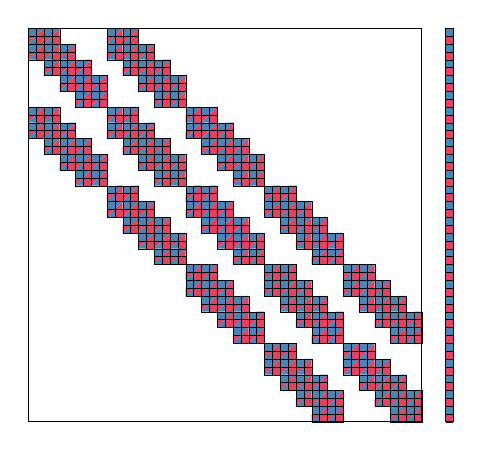
\begin{tikzpicture}

\colorlet{ca}{niceblue!80}
\colorlet{cb}{nicered!80}
\colorlet{cc}{niceorange!90}
\colorlet{cd}{niceviolet!60}

%%% Local Variables:
%%% mode: latex
%%% TeX-master: "../../diss-main"
%%% End:


\foreach \x / \y in {0/0, 0/2, 0/10, 0/12, 2/0, 2/2, 2/4, 2/10,
  2/12, 2/14, 4/2, 4/4, 4/6, 4/12, 4/14, 4/16, 6/4, 6/6, 6/8,
  6/14, 6/16, 6/18, 8/6, 8/8, 8/16, 8/18, 10/0, 10/2, 10/10,
  10/12, 10/20, 10/22, 12/0, 12/2, 12/4, 12/10, 12/12, 12/14,
  12/20, 12/22, 12/24, 14/2, 14/4, 14/6, 14/12, 14/14, 14/16,
  14/22, 14/24, 14/26, 16/4, 16/6, 16/8, 16/14, 16/16, 16/18,
  16/24, 16/26, 16/28, 18/6, 18/8, 18/16, 18/18, 18/26, 18/28,
  20/10, 20/12, 20/20, 20/22, 20/30, 20/32, 22/10, 22/12, 22/14,
  22/20, 22/22, 22/24, 22/30, 22/32, 22/34, 24/12, 24/14, 24/16,
  24/22, 24/24, 24/26, 24/32, 24/34, 24/36, 26/14, 26/16, 26/18,
  26/24, 26/26, 26/28, 26/34, 26/36, 26/38, 28/16, 28/18, 28/26,
  28/28, 28/36, 28/38, 30/20, 30/22, 30/30, 30/32, 30/40, 30/42,
  32/20, 32/22, 32/24, 32/30, 32/32, 32/34, 32/40, 32/42, 32/44,
  34/22, 34/24, 34/26, 34/32, 34/34, 34/36, 34/42, 34/44, 34/46,
  36/24, 36/26, 36/28, 36/34, 36/36, 36/38, 36/44, 36/46, 36/48,
  38/26, 38/28, 38/36, 38/38, 38/46, 38/48, 40/30, 40/32, 40/40,
  40/42, 42/30, 42/32, 42/34, 42/40, 42/42, 42/44, 44/32, 44/34,
  44/36, 44/42, 44/44, 44/46, 46/34, 46/36, 46/38, 46/44, 46/46,
  46/48, 48/36, 48/38, 48/46, 48/48}
{
  \filldraw[fill=ca,ultra thin] (0.1*\x,-0.1*\y) rectangle ++(0.1,-0.1);
}

\foreach \x / \y in {1/1, 1/3, 1/11, 1/13, 3/1, 3/3, 3/5, 3/11,
  3/13, 3/15, 5/3, 5/5, 5/7, 5/13, 5/15, 5/17, 7/5, 7/7, 7/9,
  7/15, 7/17, 7/19, 9/7, 9/9, 9/17, 9/19, 11/1, 11/3, 11/11,
  11/13, 11/21, 11/23, 13/1, 13/3, 13/5, 13/11, 13/13, 13/15,
  13/21, 13/23, 13/25, 15/3, 15/5, 15/7, 15/13, 15/15, 15/17,
  15/23, 15/25, 15/27, 17/5, 17/7, 17/9, 17/15, 17/17, 17/19,
  17/25, 17/27, 17/29, 19/7, 19/9, 19/17, 19/19, 19/27, 19/29,
  21/11, 21/13, 21/21, 21/23, 21/31, 21/33, 23/11, 23/13, 23/15,
  23/21, 23/23, 23/25, 23/31, 23/33, 23/35, 25/13, 25/15, 25/17,
  25/23, 25/25, 25/27, 25/33, 25/35, 25/37, 27/15, 27/17, 27/19,
  27/25, 27/27, 27/29, 27/35, 27/37, 27/39, 29/17, 29/19, 29/27,
  29/29, 29/37, 29/39, 31/21, 31/23, 31/31, 31/33, 31/41, 31/43,
  33/21, 33/23, 33/25, 33/31, 33/33, 33/35, 33/41, 33/43, 33/45,
  35/23, 35/25, 35/27, 35/33, 35/35, 35/37, 35/43, 35/45, 35/47,
  37/25, 37/27, 37/29, 37/35, 37/37, 37/39, 37/45, 37/47, 37/49,
  39/27, 39/29, 39/37, 39/39, 39/47, 39/49, 41/31, 41/33, 41/41,
  41/43, 43/31, 43/33, 43/35, 43/41, 43/43, 43/45, 45/33, 45/35,
  45/37, 45/43, 45/45, 45/47, 47/35, 47/37, 47/39, 47/45, 47/47,
  47/49, 49/37, 49/39, 49/47, 49/49}
{
  \filldraw[fill=cb,ultra thin] (0.1*\x,-0.1*\y) rectangle ++(0.1,-0.1);
}

\foreach \x / \y in {0/1, 0/3, 0/11, 0/13, 2/1, 2/3, 2/5, 2/11,
  2/13, 2/15, 4/3, 4/5, 4/7, 4/13, 4/15, 4/17, 6/5, 6/7, 6/9,
  6/15, 6/17, 6/19, 8/7, 8/9, 8/17, 8/19, 10/1, 10/3, 10/11,
  10/13, 10/21, 10/23, 12/1, 12/3, 12/5, 12/11, 12/13, 12/15,
  12/21, 12/23, 12/25, 14/3, 14/5, 14/7, 14/13, 14/15, 14/17,
  14/23, 14/25, 14/27, 16/5, 16/7, 16/9, 16/15, 16/17, 16/19,
  16/25, 16/27, 16/29, 18/7, 18/9, 18/17, 18/19, 18/27, 18/29,
  20/11, 20/13, 20/21, 20/23, 20/31, 20/33, 22/11, 22/13, 22/15,
  22/21, 22/23, 22/25, 22/31, 22/33, 22/35, 24/13, 24/15, 24/17,
  24/23, 24/25, 24/27, 24/33, 24/35, 24/37, 26/15, 26/17, 26/19,
  26/25, 26/27, 26/29, 26/35, 26/37, 26/39, 28/17, 28/19, 28/27,
  28/29, 28/37, 28/39, 30/21, 30/23, 30/31, 30/33, 30/41, 30/43,
  32/21, 32/23, 32/25, 32/31, 32/33, 32/35, 32/41, 32/43, 32/45,
  34/23, 34/25, 34/27, 34/33, 34/35, 34/37, 34/43, 34/45, 34/47,
  36/25, 36/27, 36/29, 36/35, 36/37, 36/39, 36/45, 36/47, 36/49,
  38/27, 38/29, 38/37, 38/39, 38/47, 38/49, 40/31, 40/33, 40/41,
  40/43, 42/31, 42/33, 42/35, 42/41, 42/43, 42/45, 44/33, 44/35,
  44/37, 44/43, 44/45, 44/47, 46/35, 46/37, 46/39, 46/45, 46/47,
  46/49, 48/37, 48/39, 48/47, 48/49}
{
  \fill[cb] (0.1*\x,-0.1*\y) -- ++(0.1,0) -- ++(-0.1,-0.1) --cycle;
  \fill[ca] (0.1*\x+0.1,-0.1*\y) -- ++(0,-0.1) -- ++(-0.1,0) --cycle;
  \draw[ultra thin] (0.1*\x,-0.1*\y) rectangle ++(0.1,-0.1);
}

\foreach \x / \y in {1/0, 1/2, 1/10, 1/12, 3/0, 3/2, 3/4, 3/10,
  3/12, 3/14, 5/2, 5/4, 5/6, 5/12, 5/14, 5/16, 7/4, 7/6, 7/8,
  7/14, 7/16, 7/18, 9/6, 9/8, 9/16, 9/18, 11/0, 11/2, 11/10,
  11/12, 11/20, 11/22, 13/0, 13/2, 13/4, 13/10, 13/12, 13/14,
  13/20, 13/22, 13/24, 15/2, 15/4, 15/6, 15/12, 15/14, 15/16,
  15/22, 15/24, 15/26, 17/4, 17/6, 17/8, 17/14, 17/16, 17/18,
  17/24, 17/26, 17/28, 19/6, 19/8, 19/16, 19/18, 19/26, 19/28,
  21/10, 21/12, 21/20, 21/22, 21/30, 21/32, 23/10, 23/12, 23/14,
  23/20, 23/22, 23/24, 23/30, 23/32, 23/34, 25/12, 25/14, 25/16,
  25/22, 25/24, 25/26, 25/32, 25/34, 25/36, 27/14, 27/16, 27/18,
  27/24, 27/26, 27/28, 27/34, 27/36, 27/38, 29/16, 29/18, 29/26,
  29/28, 29/36, 29/38, 31/20, 31/22, 31/30, 31/32, 31/40, 31/42,
  33/20, 33/22, 33/24, 33/30, 33/32, 33/34, 33/40, 33/42, 33/44,
  35/22, 35/24, 35/26, 35/32, 35/34, 35/36, 35/42, 35/44, 35/46,
  37/24, 37/26, 37/28, 37/34, 37/36, 37/38, 37/44, 37/46, 37/48,
  39/26, 39/28, 39/36, 39/38, 39/46, 39/48, 41/30, 41/32, 41/40,
  41/42, 43/30, 43/32, 43/34, 43/40, 43/42, 43/44, 45/32, 45/34,
  45/36, 45/42, 45/44, 45/46, 47/34, 47/36, 47/38, 47/44, 47/46,
  47/48, 49/36, 49/38, 49/46, 49/48}
{
  \fill[ca] (0.1*\x,-0.1*\y) -- ++(0.1,0) -- ++(-0.1,-0.1) --cycle;
  \fill[cb] (0.1*\x+0.1,-0.1*\y) -- ++(0,-0.1) -- ++(-0.1,0) --cycle;
  \draw[ultra thin] (0.1*\x,-0.1*\y) rectangle ++(0.1,-0.1);
}

\foreach \x in {0,1,...,24}
{
  \fill[ca] (5.3,-0.2*\x) rectangle ++(0.1,-0.1);
  \fill[cb] (5.3,-0.2*\x-0.1) rectangle ++(0.1,-0.1);
}

\draw (5.3,0) rectangle ++(0.1,-5);

\foreach \x in {0,1,...,50}
{
  %\draw (0.1*\x,0) -- ++(0,-5);
  %\draw (0,-0.1*\x) -- ++(5,0);
  \draw[ultra thin] (5.3,-0.1*\x) -- ++(0.1,0);
}

\draw (0,0) rectangle (5,-5);

\end{tikzpicture}


%%% Local Variables:
%%% mode: latex
%%% TeX-master: "../../diss-main"
%%% End:

}
    \end{column}
    \begin{column}{0.4\textwidth}
\resizebox{0.8\textwidth}{!}{
  \input{tikz/dofs/dgentity-unblocked-matrix}
}
\ \\[1em]
\resizebox{0.8\textwidth}{!}{
  \input{tikz/dofs/dgentity-blocked-matrix}
}

    \end{column}
  \end{columns}
\end{frame}

\begin{frame}
\frametitle{Realization in PDELab}
\begin{enumerate}[1)]
\item The ini-file
\lstinline{tutorial04.ini} holds parameters
controlling the execution.
\item Main file \lstinline{tutorial04.cc} includes the necessary C++,
DUNE and PDELab header files;
contains \lstinline{main} function;
instantiates DUNE grid objects and calls the \lstinline{driver} function
\item Function \lstinline{driver} in file \lstinline{driver.hh} instantiates
the necessary PDELab classes and finally solves the problem.
\item File \lstinline{wavefem.hh} contains the local operator classes
\lstinline{WaveFEM} and \lstinline{WaveL2} realizing the spatial
and temporal residual forms.
\end{enumerate}
\end{frame}

\begin{frame}
\bibliographystyle{plain}
\bibliography{slides04.bib}
\end{frame}

\end{document}
